%settings

\setlength{\parindent}{2ex}
\phantomsection
%text
%-Task1----------------------------------
\section{Model of the application using 3 Statechart Diagrams}
In figure \thesection.1 is presented the state chart which contains the initialization form of my application.
\begin{figure}[h!]
	\centering
	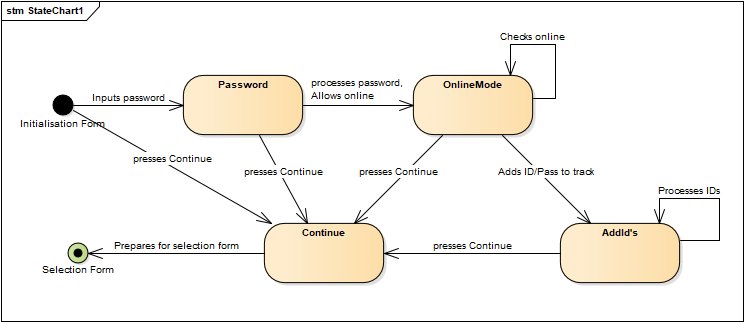
\includegraphics[keepaspectratio=true,width=\textwidth]{StateChart1}
	\caption{Initialization} 
\end{figure}
\par
In figure \thesection.2 is presented the state chart which contains the selection form of my application.
\begin{figure}[h!]
	\centering
	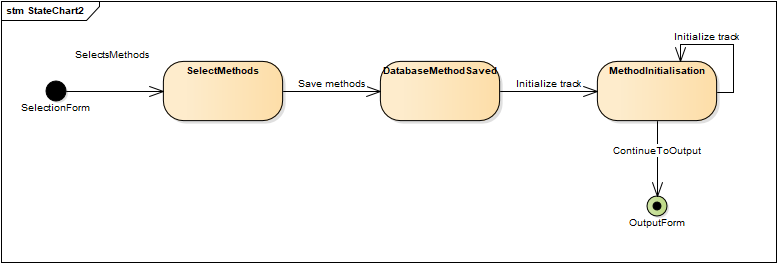
\includegraphics[keepaspectratio=true,width=\textwidth]{StateChart2}
	\caption{Selection} 
\end{figure}
\newpage
In figure \thesection.3 is presented the state chart which contains the output form of my application.
\begin{figure}[h!]
	\centering
	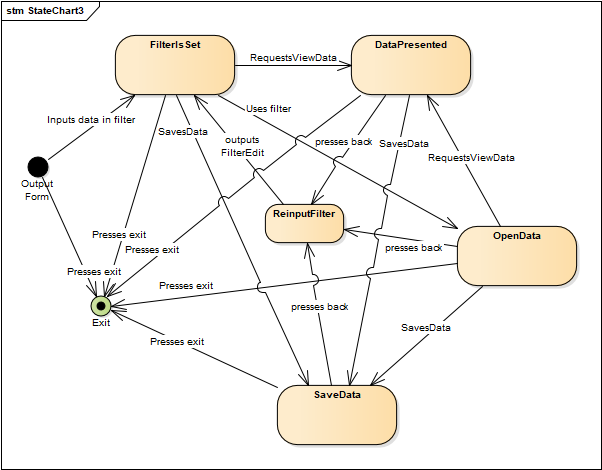
\includegraphics[keepaspectratio=true,width=\textwidth]{StateChart3}
	\caption{Output} 
\end{figure}
\par
%-Task2----------------------------------
\newpage
\section{Domain analysis of the project}
\begin{itemize}
\item[•]\textbf{ Domain description.} \par
A tracking system is used for the observing of persons or objects on the move and supplying a timely ordered sequence of location data for further processing.Regardless of the tracking technology, for the most part the end-users just want to locate themselves or wish to find points of interest. The reality is that there is no "one size fits all" solution with locating technology for all conditions and applications, therefor i added the Additional Methods to the selection.
\item[•] \textbf{Theme importance;} \par
The importance of these theme is mainly to make observations on the statistics we are provided with.Because the theme has a big spread and utilization in the read world there the importance of this theme is equal to general need.As far judging from the main functions implemented in my application the importance factors that i thought of are: \textit{to be able to trackback to a specific moment, to prevent of see access of a foreign user in the System and to monitor the how a company is prospering according to how are employees executing their tasks.} 
\item[•] \textbf{Description of existing systems(min 3);}
\begin{itemize}
\item \textbf{EXO5} (A business package that's more focused on locking down your data)\par
Specs: RemoteKill file encryption, drive lock, curfew, geolocation, logs, data export, RiskSense alerts\par
Most of its features are geared more towards an individual or company that wants to make sure that a laptop is being used for the right purposes.
Of most use is the incredibly handy RemoteKill option. This enables you to encrypt files and folders remotely if the laptop is stolen. Presets such as 'All Microsoft Outlook.pst files' make it quick and easy to secure important info. You can also add a boot sector lock to shut down the device - and both can easily be reversed if the laptop is recovered.
\item \textbf{GlassWire} free firewall software and network monitor can detect threats other miss. Download GlassWire free firewall now to protect your computer.\par 
GlassWire's network monitor visualizes your current and past network activity by traffic type, application, geographic location, all on a beautiful and easy to understand graph.
GlassWire reveals hosts that are known threats, unexpected network system file changes, unusual application changes, ARP spoofing, DNS changes, and alerts you to the problem so you can take action. GlassWire can also remotely monitor and help protect servers or other computers far away. 
\item \textbf{Norton AntiVirus} (is an anti-malware software developed and distributed by Symantec Corporation since 1991 as part of its Norton family of computer security products. It uses signatures and heuristics to identify viruses. Other features included in it are e-mail spam filtering and phishing protection.)
\end{itemize}
\item[•] \textbf{System comparison;} \par
As to what my application is capable of comparing it to other applications mentioned above it is capable of implementing the usage of other applications with additional methods and also the download/upload track method is similar to  what GlassWire is doing, but as it is a operating system track system it is less focused on tracking the exact locations and data loss prevention unless implemented in the default tracking methods.
\item[•] \textbf{Scope and objective of the chosen theme.} \par 
The scope and objective of my theme is to make a system that combines most tracking methods that are already used or adds new tracking methods which aren't yet implemented, and delivers a report easy to understand.
\end{itemize}
\clearpage
